\documentclass[letterpaper, 12pt]{article}
\raggedbottom{}
\usepackage[utf8]{inputenc}
% \usepackage[papersize={216mm,330mm},tmargin=15mm,bmargin=15mm,lmargin=15mm,rmargin=15mm]{geometry}
\usepackage[english, spanish]{babel}
\usepackage{fullpage} % changes the margin
\usepackage{graphicx}
\usepackage{enumitem}
\usepackage{chngcntr}
\usepackage{multirow}
\usepackage{parskip}
\usepackage{url}
\usepackage{booktabs} 
\counterwithin{figure}{section}
\renewcommand{\thesection}{\arabic{section}}
\renewcommand{\thesubsection}{\thesection.\arabic{subsection}}
\renewcommand{\baselinestretch}{1.5}
\usepackage{float}
\usepackage{apacite}
\usepackage{multicol}
\setlength{\columnsep}{.4cm}
\bibliographystyle{apacite}
\setlength\belowcaptionskip{10pt}
\linespread{1.5}

\begin{document}

% 									|		PRACTICA 5                 |
%  									|		GUÍA No. 7                 |

\begin{titlepage}
	\centering
	
\includegraphics[width=0.3\textwidth]{Images/logo_utb.png}\par\vspace{1cm}
	{\scshape\LARGE Universidad Tecnológica de Bolívar \par}
	\vspace{1cm}

	{\scshape\Large FÍSICA ELÉCTRICA \par}
	\vspace{.2cm}

	% chktex-file 8
	{\scshape\Large H1 - C \par}
	\vspace{1cm}
	% chktex-file 8 chktex-file 13
	\slshape {\Large \bfseries{} LAB 5 - CAMPO MAGNÉTICO EN UNA BOBINA. FUERZA MAGNÉTICA\\}
	\slshape {\small \bfseries{} Guía de laboratorio No. 7}
	\vspace{1cm}

	\slshape {\itshape{} Mauro González, T00067622 \\}
	\slshape {\itshape{} German De Armas Castaño, T00068765 \\}
	\slshape {\itshape{} Angel Vega Rodriguez, T00068186 \\}
	\slshape {\itshape{} Juan Jose Osorio Ariza, T00067316 \\}
	\slshape {\itshape{} Juan Eduardo barón, T00065901 \\}
	\vfill
	Revisado Por \\
	Gabriel Hoyos Gomez Casseres\\
	{\large \today\par}
\end{titlepage}

% ----------------------------------------------------------------------|>
\begin{multicols}{2}

	\section{Introducción}

	La fuerza magnética es una fuerza que actúa sobre objetos que se encuentran
	en presencia de un campo magnético, es decir, que es una consecuencia de la
	fuerza electromagnética, una de las cuatro fuerzas fundamentales de la
	naturaleza, y es causada por el movimiento de las cargas atómicas~\cite{FuerzaMagnetica}.

	La fuerza magnética se puede calcular utilizando la ley de Lorentz,
	que describe la fuerza que actúa sobre una carga eléctrica en movimiento
	en un campo magnético.

	{\large $F = q (v \cdot B)$}

	donde: \hfill \break{}
	\textbf{\textit{F}} es la fuerza magnética que actúa sobre la carga eléctrica,
	medida en newtons (N),
	\textbf{\textit{q}} es la carga eléctrica, medida en coulombs (C),
	\textbf{\textit{v}} es la velocidad de la carga eléctrica, medida en metros por segundo
	($\frac{m}{s}$),
	\textbf{\textit{B}} es la densidad de flujo o inducción magnética, medida en teslas (T).

	La dirección de la fuerza magnética se determina mediante la regla de la
	mano derecha: si se coloca el dedo índice en la dirección de la velocidad
	de la carga eléctrica $(v)$ y el dedo medio en la dirección del campo
	magnético $(B)$, entonces el dedo pulgar apuntará en la dirección de la
	fuerza magnética $(F)$.

	Es importante tener en cuenta que la fuerza magnética puede ser
	influenciada por la distancia entre los objetos, la intensidad y
	la orientación relativa de los campos magnéticos. Además, la fuerza
	magnética puede ser controlada y manipulada mediante la utilización de
	materiales y diseños adecuados en los objetos que interactúan magnéticamente.

	Una bobina es un componente eléctrico que está formado por un conductor
	enrollado en forma de espiral. Cuando una corriente eléctrica circula por
	la bobina, se crea un campo magnético alrededor de ella.

	Este campo magnético es perpendicular al plano de la bobina y es
	proporcional a la corriente que circula y al número de vueltas de la misma,
	además, se puede calcular su campo magnético utilizando la ley de Ampère.

	Esta quinta experiencia se enfocará en analizar cómo es el comportamiento
	de un campo magnético uniforme en el interior de un solenoide.

	% ----------------------------------------------------------------------|>
	\section{Objetivos}

	% -----------------------------------|>
	\subsection{Objetivo General}

	\begin{itemize}
		\item Identificar el funcionamiento de los circuitos para comprobar
		      la diferentes leyes que pueden intervenir en estos
		      (Leyes de Kirchhoff, Ley de malla, ley de nodos).
	\end{itemize}

	% -----------------------------------|>
	\subsection{Objetivos específicos}

	\begin{itemize}
		% \item Identificar el funcionamiento de un circuito para comprobar las leyes
		%       de Kirchhoff
		\item Comprobar en qué circunstancias se cumple la ley de malla.
		\item Precisar los voltajes correspondientes para evitar
		      recalentamientos y/o fundición de los resistores.
		\item Verificar  los factores influyentes en la ley de nodos.
	\end{itemize}

	% ----------------------------------------------------------------------|>
	\section{Preparación de la practica}

	% -----------------------------------------------------------|>
	\subsection*{Calcula el campo magnético sobre el eje de un solenoide y llega a la expresión (1).}

	El objetivo es calcular el campo eléctrico de un solenoide en un punto P situado
	en el eje del solenoide sumando el campo producido por las N espiras.

	\begin{figure}[H]
		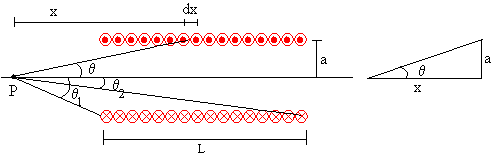
\includegraphics[width = \linewidth]{./Images/solenoide.png}
	\end{figure}

	En la figura, tenemos un corte longitudinal de un solenoide de longitud L,
	formado por N espiras iguales de radio a.

	De~\cite{CampoElectricoPorEspira} se obtuvo la expresión para calcular el campo
	magnético producido por una espira de radio $a$ en un punto $P$ de su eje
	distante $X$.

		% chktex-file 3
		{\large $B = \displaystyle\frac{\mu_0 i a^2}{2 \left(\sqrt{a^2 + x^2}\right)^3}$}

	Todas las espiras del solenoide producen sobre P un campo que tiene la misma
	dirección y sentido, pero distinto módulo, dependiendo de la distancia $X$ al
	punto P.

	El número de espiras que hay en el intervalo comprendido entre
	$x$ y $x+dx$ es $dn = N \cdot \frac{dx}{L}$

	Estas espiras producen en P un capo que es el producto del campo producido por
	una espira por el numero de espiras.

		{\large $dB = \frac{\mu_0 i a^2}{2 \left(\sqrt{a^2 + x^2}\right)^3} \cdot \frac{N}{L} dX$}

	Para integrar, tenemos que hacer el cambio de variable $a = \tan\theta$ y
	teniendo en cuenta que, {\large $1 + \tan^{2}\theta = \frac{1}{\cos^{2}\theta}$},
	simplificamos la integral

		% {\large $B = \frac{\mu_0 i N}{2L} \int_{\theta_1}^{\theta_2} -\sin\theta \cdot \,d\theta$}

		{\large $B = \frac{\mu_0 i N}{2L} \Bigg[ \displaystyle\int_{\theta_1}^{\theta_2} -\sin\theta \cdot \,d\theta \Bigg]$}

		{\large $ = \frac{\mu_0 i N}{2L} \left(\cos\theta_2 - \cos\theta_1\right)$}

	Si el solenoide es muy largo comparado con su radio $a$ y si el punto $P$ esta
	situado en el centro, tendremos que $\theta_1 \rightarrow \pi$ y
	$\theta_2 \rightarrow 0$. El campo $B$ vale entonces:

	{\large $B = \frac{\mu_0 i N}{L}$}

	Fuente:~\cite{CampoElectricoSolenoide}

	% -----------------------------------------------------------|>
	\subsection*{Demuestra la expresión (3) y (4) realizando los esquemas necesarios para las corrientes, el
		campo y la fuerza resultante}

	{\large $Fm = IL \times B$}

	$Fm = I_e L B \sin(180) = 0$

	$Fm = I_e L B \sin(0) = 0$

	$Fm = I_e L \times B = I_e L B \sin(90) = I_e L $

	$L = d$

	$Fm = I_e d B$

	$Fx = Wx \rightarrow F = W$

	$Fm = I_e d B \rightarrow W = I_e d B$

	$B = \frac{W}{I_e d}$

	% ----------------------------------------------------------------------|>
	\section{Resumen del procedimiento}

	Se armara el circuito con el fin de establecer una corriente directa en
	la bobina, se encenderá y se ajustara a una corriente de 4A, para saber
	en que dirección se encuentra el campo magnético se colocara una brújula
	cerca del núcleo del solenoide, tal como se muestra coloque la espira
	dentro del solenoide  y se armara el circuito para alimentarla.

	Se encenderán las dos fuentes que alimentan la espira y la bomba y se
	aumentara gradualmente el voltaje en la fuente de la espira hasta que se
	obtenga una corriente de 1A.

	Luego se desviara la espira y se colocara en la balanza hilos de densidad
	y masa lineal y se ajustara la corriente haga que la balanza llegue al
	equilibrio, se registrara la masa del hilo, la corriente tanto de la
	espira como de la bobina y se hará el mismo procedimiento para otros
	valores de la masa del hilo. Sin olvidar de registrar los datos de la
	bobina y la espiral.

\end{multicols}

\newpage

\bibliography{./Bibliography/bibliography.bib}

\end{document}